\graphicspath{ {images/mat/} }
\section{Фоновые задачи} \label{sec:mass_async_task}

Раздел <<Фоновые задачи>> доступен из меню <<Мой профиль>> пользователю, у которого имеется хотя бы одна роль в рамках какого-либо университета. Конкретная задача в списке доступна её автору только если у пользователя есть любое право в рамках привязанного к задаче университета.

\begin{figure}[H]
	\center{
\includegraphics[width=1\linewidth]{my_mats}}
	\caption{Переход в раздел <<Фоновые задачи>>}
	\label{img:employee:my_dumps}
\end{figure}

Задачи в данном разделе появляются в результате выполнения пользователем массовых операций, таких как:
\begin{itemize}
	\item приглашение пользователей на платформу (только списком);
	\item зачисление пользователей на курс; 
	\item изменение режима прохождения курса;
	\item отчисление пользователей с курса;
	\item назначение ролей в рамках курса;
\end{itemize}

В целом данный раздел также представляет собой табличные данные с возможностью фильтрации, поиска, сортировки и выгрузки.
Более подробно эти возможности описаны в подразделе~\ref{sec:datatables}. Таблица с фоновыми задачами содержит специальную колонку <<подробнее>> (\vcenteredinclude[height=25px]{verbose}), позволяющую развернуть строку таблицы. В развёрнутой строке содержатся такие данные, как:
\begin{itemize}
	\item текстовый статус задачи (в процессе, завершено, завершено с ошибками)
	\item ссылки на CSV"=файлы с успешными и неуспешными результатами операций.
\end{itemize}

CSV"=файлы, загружаемые по ссылке из развёрнутой строки соответсвуют универсальному формату данных (см. раздел~\ref{sec:csv_format}) и пригодны для повторной загрузки в форму, создавшую данную операцию (если операция создана с помощью загрузки CSV"=файла). Помимо столбцов, описанный в разделе~\ref{sec:csv_format}, список неуспешных результатов, также содержит столбец с сообщениями об ошибках для каждого неуспешного результата (последний столбец). При повторной загрузке CSV"=файла в формы этот столбец можно как удалить из файла, так и оставить в файле, на повторную загрузку это не повлияет.

Статус, помимо текстового описания в развёрнутой строке также кодируется цветом строки:
\begin{itemize}
	\item жёлтый "--- задача в процессе;
	\item зелёный "--- задача успешно завершена;
	\item красный "--- задача завершена с ошибками.
\end{itemize}

Легенду для цветов таблицы можно также получить, нажав на значок \vcenteredinclude[height=25px]{legend} вверху таблицы.

Пример таблицы с задачами приведён на рис.~\ref{img:mat:list}. Строки с ID 36 и 35 развёрнуты для просмотра подробностей. Задачи с ID 35 и 38 завершены успешно, с ID 36 и 39 "--- с ошибками. Задачи с ID 32, 33 и 34 находятся в процессе выполнения.

\begin{figure}[H]
	\center{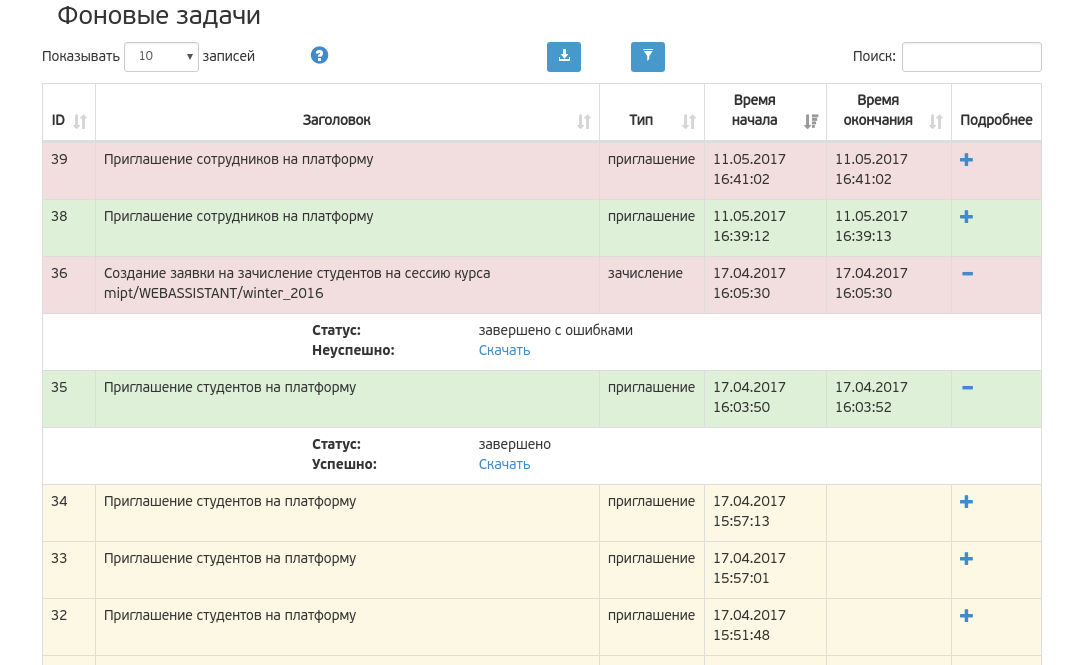
\includegraphics[width=1\linewidth]{list}}
	\caption{Список фоновых задач}
	\label{img:mat:list}
\end{figure}
